\label{Chapter:BYOL}

\section{Motivation}

We have shown how contrastive methods rely on comparing different views of the same image with views of other images, considering the ones from the same image as positive and the rest as negative samples. This is why they are called \emph{self-supervised} methods.

Self-supervised methods build upon the cross-view prediction framework, i.e., learning representations by predicting different views (or data augmentations) of the same image. This could lead the frameworks to collapsed representations, such as a constant representation for any view of the image can easily help us to identify objects, but it is useless for downstream tasks.

The methods presented earlier, which use contrastive learning, avoid this problem by trying to discriminate between positive and negative views, as we have already explained.

However, some papers (e.g. \cite{caron2019deep}) have already raised the following question:

\begin{quote}
    \centering
\emph{ Is the use of negative samples necessary to avoid collapsing? }. 
\end{quote}
This question is studied in \cite{grill2020bootstrap}, paper that presents an algorithm that we will be deeply explaining.

The first solution that comes to mind to prevent the collapsing problem would be to use a randomly initialized network to produce the targets of the predictions. As it is probably expected, due to its randomness, it does not produce good representations for downstream tasks. Nonetheless, the representations obtained were empirically much better than initial fixed representation, so it could be interesting to refine this representation in order to make it better for the later tasks. This is the intuitive idea behind \emph{Boostrap your own latent (BYOL)} \citep{grill2020bootstrap}.

\section{BYOL Algorithm}

BYOL's algorithm has certain similarities with the SimCLR framework that we presented in Chapter \ref{Chapter:SimCLR}. The goal of this framework is to learn a representation for an input. In this case, the representation will be noted as $y_\theta$. 

For this purpose, two neural networks are used:
\begin{itemize}
\item An \emph{online} network defined by a set of weights $\theta$.

\item A \emph{target} network, defined by a different set of weights $\upxi$.
\end{itemize}

They both have the same structure, composed of three stages:
\begin{enumerate}
\item An encoder $f_\gamma$,
\item A projector $g_\gamma$,
\item A predictor $q_\gamma$,
\end{enumerate}
where $\gamma \in \{\theta,\upxi\}$. In the online network, despite their different name, the projector $g_\theta$ and the predictor $q_\theta$ have the same architecture.

\begin{remark}
The projector $g_\gamma$ is used because in SimCLR \citep{chen_simple_2020} is proven empirically that this projection improves the general performance of the framework.
\end{remark}

The \emph{difference} between them is that the target network provides the regression targets to train the online network, and its parameters $\upxi$ are an exponential moving average\footnotemark of the online parameters $\theta$. Mathematically, given a rate decay $\tau \in [0,1]$, after each training step $\upxi$ is updated as follows:
\[
\upxi \leftarrow \tau \upxi + (1-\tau)\theta    
\]

%------------- Footnotemark
\footnotetext{A moving average is a calculation to analyze data points by creating a series of averages in different subsets of the data. }
%----------------------

Having presented the networks and its structure, the following steps are followed in BYOL's framework:

\begin{enumerate}
\item The input that both networks receive is different, even if it comes from the same image. As in SimCLR, given an input image $x$ and two distributions of data augmentation for images, $\mathcal T, \mathcal T'$, two views are produced from $x$ to get $v = t(x), v' = t'(x)$ where $t \sim \mathcal T $ and $t' \sim \mathcal T'$.

\item Each produced view is passed to one of the networks. In particular, the first view $v$ is passed to the online network, and follows the next steps:
\[
x \longmapsto v = t(x) \longmapsto y_\theta = f_\theta(v) \longmapsto z_\theta =  g_\theta(y_\theta)    
\]
where $f_\theta,g_\theta$ are the ones that we mentioned before in the structure of each networks. This online network outputs $y_\theta$ and $z_\theta$.

In a similar process, the the target network is passed the second view $v'$, which follows the next steps:
\[
x \longmapsto v' = t'(x) \longmapsto y_\upxi' = f_\upxi(v') \longmapsto z_\upxi' = g_\upxi(y_\upxi')   
\]
where, again, $f_\upxi,g_\upxi$ are the ones mentioned before.


\item Then, using the online network, a prediction $q_\theta(z_\theta)$ is produced. Remark that the prediction is \emph{only} applied to the online network.

\item Having $q_\theta(z_\theta)$ in the online network and $z_\upxi'$ in the target network, they are both $\ell_2$-normalized to
\[
\overline{q_\theta}(z_\theta) = \frac{q_\theta(z_\theta)}{\norm{q_\theta(z_\theta)}} \quad \text{and} \quad \overline{z_\upxi'} = \frac{z_\upxi'}{\norm{z_\upxi'}}. 
\]

\item \label{BYOL:not:last} Now, we can define the mean squared error between the normalized prediction $\overline{q_\theta}(z_\theta)$ and the normalized projection $\overline{z_\upxi'}$:
\[
\mathcal L_{\theta,\upxi} = \norm{\overline{q_\theta}(z_\theta) - \overline{z_\upxi'}}_2^2. 
\]

\item If we stopped in the step \ref{BYOL:not:last}, the framework would be asymmetric between the two networks, since the projection is performed in one of the views, $v$ but not in the other one, $v'$. To fix this, the process described is repeated except that now $v'$ is the input of the online network and $v$ is the input of the target network, producing a new loss $\tilde{\mathcal L}_{\theta,\upxi}$. The final loss is computed as:
\begin{equation}\label{Loss:BYOL}
\mathcal L_{\theta,\upxi}^{\operatorname{BYOL}}     = \mathcal L_{\theta,\upxi} + \tilde{\mathcal L}_{\theta,\upxi} 
\end{equation}
\end{enumerate}

The loss in Equation \eqref{Loss:BYOL} is the one that must be optimized stochastically. Furthermore, since we have expressed $\upxi$ depends on $\theta$, if $\eta$ is the learning rate that we want to apply, the optimization problem can be expressed as follows:
\[
\begin{cases}
    \theta \gets \operatorname{optimizer}\left(\theta,\nabla_\theta \mathcal L_{\theta,\upxi}^{\operatorname{BYOL}},\eta \right), \\
    \upxi \gets \tau \upxi + (1-\tau)\theta 
\end{cases}
\]

The framework can be summarized in the following figure:
\begin{figure}[H]
    \centering 
    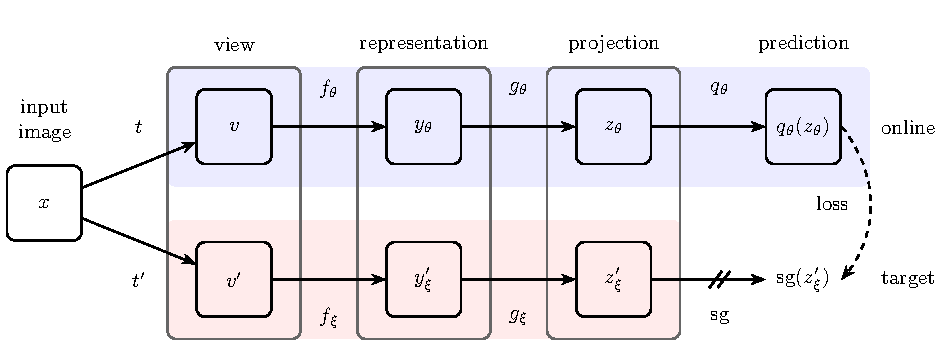
\includegraphics[scale=0.8]{Archi-BYOL.pdf}
    \caption{Image from \citep{grill2020bootstrap}. Overview of Bootstrap Your Own Latent Framework. }
\end{figure}

The \emph{sg (stop gradient)} indicates that, at that point, the gradient is not propagated back. 

After the whole model has been fully trained, both the projection $g_\theta$  and the prediction $q_\theta$ are discarded, since what it is interesting for us is the representation of the input, and it is what it will be used in downstream tasks.

Some considerations have to be made about this framework:
\begin{enumerate}
    \item About data augmentation: In BYOL,it is not important if the model learns about the histogram of the image, since we want ot keep any information captured by the target representation into its online network. In the original paper, it is empirically shown how BYOL is more robust to the choice of the image augmentations than SimCLR.

    \item Since the weights of the target network $\upxi$ depend on the weights of the online network $\theta$ by a parameter $\tau$, the first mentioned weights $\upxi$ represent a delayed and stable version of $\theta$. Actually, if the decay rate $\tau$ is $1$, we never update $\upxi$, and if $\tau = 0 $, then the weights of the target network are always being updated. This way, a trade-off is tablished between updating $\upxi$ too often or too slowly. Empirically, it has been shown that the most adequate values that yield to more stable results are $\tau \in [0.9,0.999]$.
\end{enumerate}

\section{Results obtained by this framework}

In this framework, the impact of the batch size varies respect to the importance that it had in SimCLR. In contrast with BYOL's framework, in SimCLR we were using negative samples in our network to learn how to produce the representations. Because of this, BYOL's is expected to be more robust to smaller batch sizes. 

It is empirically shown that the regularization of the weights is crutial in the self-supervised setting. The experiments in the paper showed that removing the weight decay regularization led to model divergence.


BYOL achieved the state-of-art performance results in the linear evaluation. This is, again, one of the most interesting parts since it helps us to evaluate how good the representations that our model create are.

\begin{table}[H]
    \label{table:best:first:simclr}
\centering
\begin{tabular}{llrrr}
Method & Architecture & Params & Top-1 & Top 5 \\ \hline
SimCLR & ResNet-50($2\times)$ & 94M & 74.2 & 92.0 \\
BYOL & ResNet-50($2\times)$ & 94M & \textbf{77.4} & \textbf{93.6} \\
SimCLR & ResNet-50($4\times)$ & 375M & 76.5& 93.2 \\
BYOL & ResNet-50($4\times)$ & 375M & \textbf{79.6}& \textbf{94.8} \\
\end{tabular}
\caption{Comparison between SimCLR and BYOL Top1 and Top5 accuracies using the same architectures on the ImageNet dataset.}
\end{table}

BYOL also outperformed other models such as \emph{MoCo} \citep{he2020momentum} and a second version of the Contrastive Predictive Coding framework \citep{hénaff2020dataefficient}, but they have not been included in the table since they are not deeply studied in this work.